\chapter{Monte Carlo: estimators, errors and Heston simulation}
\label{cap:mc}

When no formula exists (path-dependent exotics) we \emph{simulate}: we generate many scenarios of the underlying,
compute the payoff on each, and take the average. This chapter explains:
\begin{itemize}
\item how the error of a Monte Carlo (MC) estimate is measured;
\item how to decide whether an MC estimate ``agrees'' with a formula, and what a passed test really means;
\item why statistical error and discretization error must be treated separately;
\item how to simulate the Heston model, which is more delicate than it looks.
\end{itemize}
Variance reduction techniques and the systematic convergence study are in Chapter~\ref{cap:benchmark}.

\section{The estimator and its standard error}
The price is $V=\DF\,\E[g]$, where $g$ is the payoff (a random variable). With $N$ independent scenarios
$g_1,\dots,g_N$:
\begin{equation}\label{eq:mc-stima}
\hat V=\DF\,\bar g,\qquad\bar g=\frac1N\sum_{i=1}^Ng_i .
\end{equation}
The standard error (SE) is the standard deviation of the estimator, estimated from the same data:
\begin{equation}\label{eq:mc-se}
\SE=\DF\,\frac{s_g}{\sqrt N},\qquad s_g^2=\frac1{N-1}\sum_{i=1}^N(g_i-\bar g)^2 .
\end{equation}

\textbf{Why it works.} The $g_i$ are independent and identically distributed, so $\Var\bar g=\Var g/N$. By the
\textbf{central limit theorem}, if $\Var g<\infty$,
\[
\sqrt N\,(\bar g-\E g)\ \longrightarrow\ \N(0,\Var g).
\]
Hence $\hat V$ is approximately Gaussian around $V$ with standard deviation $\SE$, and a 95\% confidence interval is
$\hat V\pm1.96\,\SE$.

\begin{idea}[title={\texorpdfstring{Key idea: the $N^{-1/2}$ law}{Key idea: the N\textasciicircum(-1/2) law}}]
The error decreases like $1/\sqrt N$: halving it takes 4 times as many scenarios, gaining one decimal digit takes 100
times as many. There are two ways to reduce the error: increase $N$, or reduce $s_g$ (variance reduction). On a
log-log plot of error against $N$ the slope is $-\tfrac12$; the experimental check of this slope is in
Chapter~\ref{cap:benchmark}.
\end{idea}

\begin{attenzione}[title={Finite variance: why we simulate puts}]
The central limit theorem requires finite variance.
\begin{itemize}
\item Puts have a bounded payoff ($0\le g\le K$): the variance is always finite.
\item Calls require $\E F_T^2<\infty$. In Heston this moment can explode (Section~\ref{sec:heston-code}); in SABR it
is infinite for a large part of the parameter space (Chapter~\ref{cap:sabr}).
\end{itemize}
With infinite variance the estimated SE jumps from one seed to the next and is not reliable. Project rule: we
simulate puts and obtain calls by parity, but only with schemes that preserve the martingale property
(Section~\ref{sec:qe-m}).
\end{attenzione}

\section{The ``within 3 standard errors'' test}
\subsection{The test and false alarms}
To check an MC estimate against an exact value $V_{\text{ref}}$ (whose error is negligible relative to the SE) we
require
\begin{equation}\label{eq:test-3se}
|z|\le3,\qquad z=\frac{\hat V-V_{\text{ref}}}{\SE}.
\end{equation}
If the code is correct and the scheme is unbiased, $z$ is approximately $\N(0,1)$. The test still fails with
probability
\[
\PP(|Z|>3)=2\Phi(-3)=0.27\%,
\]
that is, about once in 370.

\subsection{Multiple tests}
With $m$ independent tests, the probability that at least one fails with correct code is
\begin{equation}\label{eq:test-multipli}
\PP(\text{at least one failure})=1-0.9973^m .
\end{equation}

\begin{esempio}[title={Example: how often a correct gate fails}]
\begin{itemize}
\item $m=20$: $1-0.9973^{20}=5.3\%$.
\item $m=24$ (the QE gate of this chapter): about 6\%.
\item $m=100$: 24\%.
\end{itemize}
An isolated failure is therefore not automatically a bug. It must, however, \emph{always} be diagnosed: reproduce it
(the seed is fixed), check whether its sign and size are compatible with noise, and repeat with more scenarios.
\end{esempio}

Equation \eqref{eq:test-multipli} holds for independent, unbiased tests. In practice often neither assumption is
exact.
\begin{itemize}
\item \textbf{Correlated tests.} If all strikes are priced on the same paths, their errors are correlated.
\item \textbf{Small deterministic offsets.} If the reference itself is an approximation (for example Hagan's
formula in Chapter~\ref{cap:sabr}), the mean of $z$ is not zero.
\end{itemize}
The actual false-alarm rate is then measured by repeating the gate with many fresh seeds. In Chapter~\ref{cap:sabr},
for example, 21 correlated comparisons give 4.0\% of failed seeds, against 5.5\% from the independent-test formula.

\subsection{Power of the test}
If the scheme has a genuine systematic error (bias) $b$, then $z\approx\N(b/\SE,1)$ and the test detects it with
probability
\begin{equation}\label{eq:potenza}
\PP(|z|>3)\approx\Phi\Big(\frac{|b|}{\SE}-3\Big):
\end{equation}
50\% if $b=3\,\SE$, 97.7\% if $b=5\,\SE$. The test only ``sees'' biases larger than the noise. A passed test is
statistical evidence at that resolution, not a proof that there is no bias.

\subsection{Practical rules}
\begin{itemize}
\item \textbf{Two independent MC estimates} are compared with $\sqrt{\SE_1^2+\SE_2^2}$ in the denominator.
\item \textbf{Fixed seed, declared in advance.} Every result reports the generator seed and is reproducible bit for
bit. Changing the seed until the test passes is equivalent to loosening the tolerance and is forbidden.
\item \textbf{Anti-selection check.} The gate is repeated with fresh seeds, declared before running it, and the
distribution of the $z$ values is inspected: mean close to 0, standard deviation close to 1.
\end{itemize}

\section{Two different errors: bias and noise}
When the model cannot be simulated exactly, time is discretized with a step $\Delta$. The total error then has two
components:
\begin{itemize}
\item the \textbf{discretization bias} $b(\Delta)=\E[\hat V_\Delta]-V$, which depends on $\Delta$ and does \emph{not}
shrink as $N$ grows. For a scheme of \emph{weak order} 1, $b(\Delta)\approx c\Delta$;
\item the \textbf{statistical noise}, with standard deviation $\sigma_g/\sqrt N$.
\end{itemize}
The mean squared error is the sum of the two squares:
\begin{equation}\label{eq:mse}
\mathrm{MSE}=b(\Delta)^2+\frac{\sigma_g^2}{N}\approx c^2\Delta^2+\frac{\sigma_g^2}{N}.
\end{equation}

\begin{perche}[title={Why halving the step means quadrupling the scenarios}]
Neither term should dominate: the effort spent on the other would be wasted. Keeping the two terms proportional,
$c\Delta\propto\sigma_g/\sqrt N$, that is, $N\propto\Delta^{-2}$. If $\Delta$ is halved, the bias halves; for the
noise to halve as well, 4 times as many scenarios are needed. This is the Duffie--Glynn rule for order-1 schemes.
\end{perche}

\section{The step-halving test with common random numbers}
\label{sec:halving}
\subsection{The idea}
To check the discretization bias without knowing the exact price, we compare two step sizes:
\[
d=\hat V_\Delta-\hat V_{\Delta/2}.
\]
To reduce the noise of this difference we use \textbf{common random numbers} (CRN): the two simulations use the
\emph{same} shocks. On the coarse step the increment is built from two fine increments:
\[
Z^{\text{coarse}}=\frac{Z_1+Z_2}{\sqrt2}\sim\N(0,1).
\]
The two prices are then strongly correlated, and their difference has a much smaller variance than either of them.

\subsection{\texorpdfstring{Why a ``within 3~SE'' test on $d$ fails for an order-1 scheme}{Why a ``within 3 SE'' test on d fails for an order-1 scheme}}
It is tempting to require $|d|\le3\,\SE_d$, where $\SE_d$ is the standard error of the difference. This is a mistake
in the set-up.

\textbf{Step 1: the mean of $d$.} For an order-1 scheme,
\[
\E[d]=b(\Delta)-b(\Delta/2)\approx c\Delta-c\tfrac\Delta2=\tfrac12c\Delta\ne0 .
\]
$d$ does not have zero mean \emph{by construction}: the bias is a property of the scheme, not a defect of the code.

\textbf{Step 2: the variance of $d$.} With CRN the two paths differ only by the path-by-path discretization error,
which is small. $\SE_d$ is therefore much smaller than the SE of a single price, and it falls like $1/\sqrt N$.

\textbf{Step 3: the ratio.} $\E[d]/\SE_d$ grows like $\sqrt N$. With enough scenarios the test ``sees'' the
legitimate bias of the scheme and fails even if the code is perfect.

\begin{idea}
A test $|d|\le3\,\SE_d$ with CRN is an \emph{identity} only for a scheme whose bias is negligible relative to
$\SE_d$ (for example an order-2 scheme). For an order-1 scheme the right test does not ask ``$d=0$'', but ``$d$ is
small'' and ``the bias behaves like $c\Delta$''.
\end{idea}

\subsection{The replacement test: size and order}
\begin{enumerate}
\item \textbf{Size check.} By Richardson, $b(\Delta)\approx2d$. We require $|d|\le0.1\,\SE_{\text{gate}}$, where
$\SE_{\text{gate}}$ is the SE of the main gate. The bias is then $\lesssim0.2\,\SE_{\text{gate}}$, and by
\eqref{eq:potenza} the false-alarm rate of each comparison rises at most from 0.27\% to about 0.33\%.
\item \textbf{Order check.} We compute $M\big(\hat V_{1/M}-\hat V_{1/2M}\big)$ for several $M$ (number of steps). If
the scheme is of order 1, $d\approx c/(2M)$ and the quantity is flat in $M$.
\end{enumerate}
Chapter~\ref{cap:sabr} applies this test to the SABR log-Euler scheme: the ``3~SE'' test with CRN gives $z$ values
down to $-7.96$ with correct code, while the order check is flat and the size check is satisfied at all expiries.

\section{Simulating Heston: the negative-variance problem}
The most obvious scheme is Euler on the variance:
\[
v_{n+1}=v_n+\kappa(\theta-v_n)\Delta+\xi\sqrt{v_n\Delta}\,Z_v .
\]
With realistic parameters (Feller violated) the variance often lives close to zero. A step with a sufficiently
negative $Z_v$ takes it below zero, and at the next step $\sqrt v$ does not exist. A ``fix'' is needed, and the fix
changes the price.

\subsection{Euler with full truncation}
We work on the state $x_t=\ln(F_t/F)$ and build the forward shock with Cholesky \eqref{eq:cholesky}:
\begin{align}
Z_F&=\rho Z_v+\sqrt{1-\rho^2}\,Z_\perp,\label{eq:euler-zf}\\
v_{n+1}&=v_n+\kappa(\theta-v_n^+)\Delta+\xi\sqrt{v_n^+\Delta}\,Z_v,\label{eq:euler-ft}\\
x_{n+1}&=x_n-\tfrac12v_n^+\Delta+\sqrt{v_n^+\Delta}\,Z_F .\label{eq:euler-x}
\end{align}
The state $v_n$ may be negative, but only $v_n^+=\max(v_n,0)$ enters the formulas.

\begin{perche}[title={Why full truncation in particular}]
When the true process reaches zero, it has zero volatility and a positive drift $\kappa\theta$ that pushes it back
up. Full truncation copies exactly this behavior: with $v_n<0$ the next step has zero variance and drift
$\kappa\theta$.

The alternatives add spurious variance: \emph{absorption} (resetting $v=0$) and \emph{reflection} ($v\to|v|$). In the
literature (Lord, Koekkoek and van Dijk), on the BK-2 set ATM with 20 steps per year, the bias is 0.050 for full
truncation, 2.102 for absorption and 4.360 for reflection. All the fixes overprice the call; full truncation much
less so.
\end{perche}

\begin{idea}[title={The forward stays an exact martingale}]
In \eqref{eq:euler-x} the coefficient $v_n^+$ is known at the start of the step and $Z_F$ is independent of it. By the
moment generating function of the normal, $\E[e^{aZ}]=e^{a^2/2}$:
\[
\E\big[e^{x_{n+1}-x_n}\mid\mathcal F_{t_n}\big]
=e^{-\frac12v_n^+\Delta}\,\E\big[e^{\sqrt{v_n^+\Delta}\,Z_F}\big]
=e^{-\frac12v_n^+\Delta}e^{\frac12v_n^+\Delta}=1,
\]
exactly, for any $\Delta$. If the coefficient used $v_{n+1}$ or an average, this property would be lost.
\end{idea}

\subsection{The Euler bias}
The bias of Euler with full truncation is empirically of order 1 ($b\approx c\Delta$). There is, however, no theorem
for $\nu_F<1$: weak order 1 requires smooth coefficients, and $\sqrt v$ is not Lipschitz at zero. It is also
advisable to keep $\kappa\Delta<1$, otherwise the factor $(1-\kappa\Delta)^n$ in the mean oscillates.

The bias is large exactly where it is least wanted: with Feller strongly violated, the probability mass piles up
near zero, where the discretization is worst.

\begin{figure}[htbp]
\centering
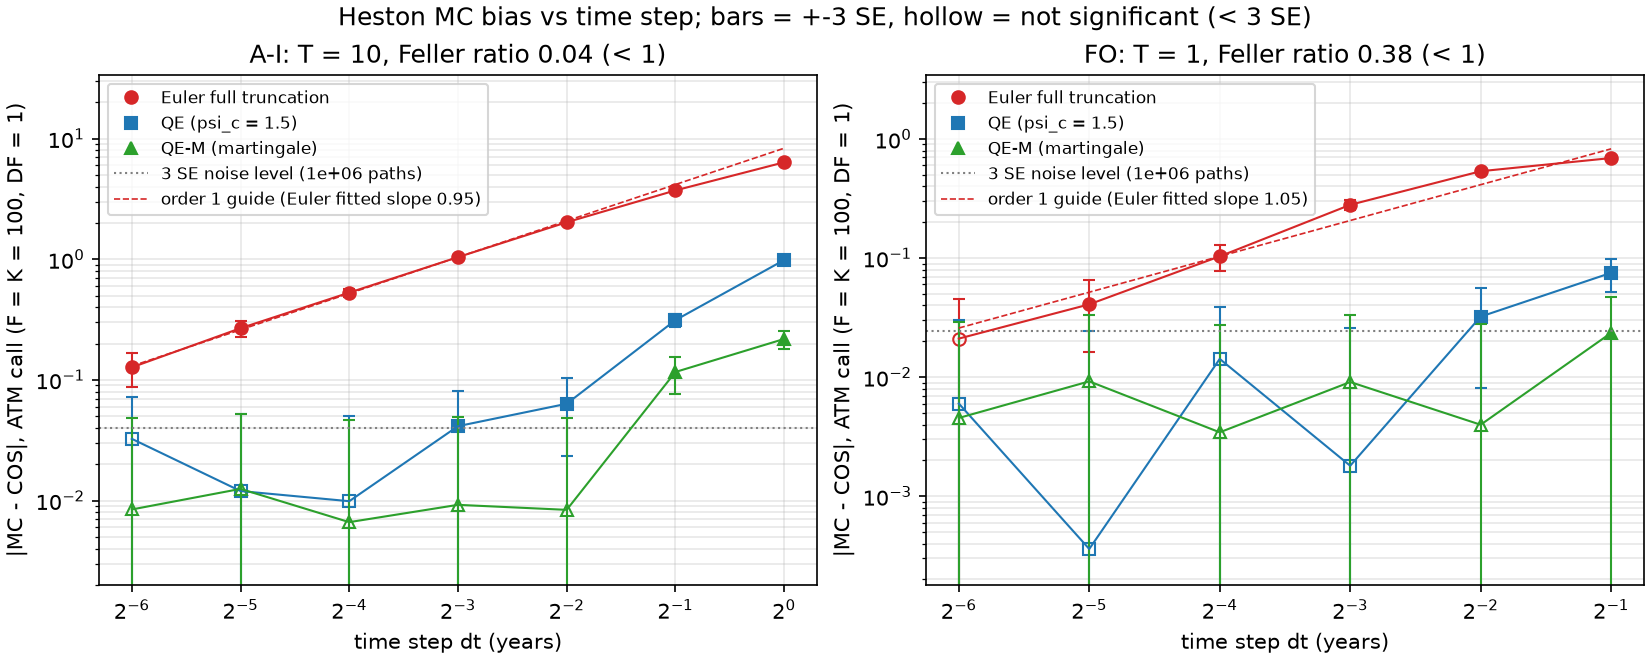
\includegraphics[width=\textwidth]{heston_euler_bias.png}
\caption{Heston Monte Carlo bias against the time step, ATM call ($F=K=100$, $\DF=1$), $10^6$ paths per point. Bars
$\pm3\,\SE$; open symbols mark non-significant points ($<3\,\SE$). Left: set A-I ($T=10$, $\nu_F=0.04$). Right: set
FO ($T=1$, $\nu_F=0.38$). The dashed red line is an order-1 guide.}
\label{fig:heston-euler-bias}
\end{figure}

Figure~\ref{fig:heston-euler-bias} shows the bias $|\text{MC}-\text{COS}|$ of the three schemes of this chapter
against $\Delta$, on a log-log scale.
\begin{itemize}
\item \textbf{Euler, set A-I} ($\nu_F=0.04$): $+6.368$ at $\Delta=1$, $+0.268$ at $\Delta=1/32$ (19.6~SE), $+0.127$
at $\Delta=1/64$. The decrease is monotonic and always significant; the estimated slope is 0.945.
\item \textbf{Euler, set FO}: $+0.692$ at $\Delta=\tfrac12$, $+0.041$ at $\Delta=1/32$ (5.0~SE), $+0.021$ at
$\Delta=1/64$ (2.6~SE, by now inside the noise). Estimated slope 1.054.
\item \textbf{QE and QE-M} (below) have much smaller biases already at coarse steps and drop into the noise much
earlier.
\end{itemize}
The acceptance criterion for the figure is: the Euler bias exceeds 3~SE at the coarsest step and decreases
monotonically until it enters the noise band. No slope is claimed inside the noise.

\begin{progetto}[title={In the qpricer project: comparison with the literature}]
Andersen publishes, for set A-I, $K=100$, the bias of Euler with full truncation: $+6.394$ at $\Delta=1$, $+1.051$ at
$\Delta=1/8$, $+0.243$ at $\Delta=1/32$. The project measures $+6.368$, $+1.042$, $+0.268$: the scheme is the same.

At the gate step ($\Delta=1/32$, ${2\times10^5}$ paths, puts with $K=70,100,140$) Euler on set A-I measures
$z=+4.39$, $+5.08$ and $+1.28$. This was predicted before running the test: at $K=100$ the published bias (0.243) is
larger than $3\,\SE\approx0.17$ (SE 0.058). This is why Euler is \emph{not} subjected to the 3~SE test: it is the
scheme, not a bug, and it goes into Figure~\ref{fig:heston-euler-bias}.
\end{progetto}

\section{Andersen's QE scheme}
\subsection{The idea}
Instead of taking an Euler step on the variance, we \emph{sample} $v_{n+1}$ from a simple distribution that has
exactly the same mean and variance as the true law (``quadratic--exponential'', QE).

\textbf{Step 1: the exact moments.} Conditional on $v_n$, the true law of $v_{n+1}$ is a scaled non-central
chi-squared. Its first two moments are, with $E=e^{-\kappa\Delta}$:
\begin{equation}\label{eq:qe-momenti}
m=\theta+(v_n-\theta)E,\qquad
s^2=\frac{v_n\xi^2E(1-E)}{\kappa}+\frac{\theta\xi^2(1-E)^2}{2\kappa}.
\end{equation}
Their relative dispersion is $\psi=s^2/m^2$. It is largest at $v_n=0$, where it equals $1/\nu_F$: the more Feller is
violated, the more dispersed the law of $v_{n+1}$ is relative to its mean.

\textbf{Step 2a ($\psi\le\psi_c$, variance away from zero): square of a Gaussian.} We set $v_{n+1}=a(b+Z_v)^2$. This
variable has mean $a(1+b^2)$ and variance $2a^2(1+2b^2)$. Imposing mean $m$ and variance $s^2$, with $y=b^2$:
\[
\psi(1+y)^2=2(1+2y)\iff y^2+2y\Big(1-\frac2\psi\Big)+1-\frac2\psi=0 .
\]
The non-negative root is
\begin{equation}\label{eq:qe-quad}
b^2=\frac2\psi-1+\sqrt{\frac2\psi}\sqrt{\frac2\psi-1},\qquad a=\frac{m}{1+b^2}.
\end{equation}
The discriminant is non-negative only if $\psi\le2$.

\textbf{Step 2b ($\psi>\psi_c$, variance near zero): atom at zero plus exponential.} With probability $p$ we set
$v_{n+1}=0$; otherwise we draw an exponential with parameter $\beta$. The mixture has mean $(1-p)/\beta$ and variance
$(1-p^2)/\beta^2$, hence $\psi=(1+p)/(1-p)$ and
\begin{equation}\label{eq:qe-exp}
p=\frac{\psi-1}{\psi+1},\qquad\beta=\frac{1-p}{m}.
\end{equation}
This requires $\psi\ge1$. We sample by inverting the distribution function with $U_v=\Phi(Z_v)$:
\[
v_{n+1}=\begin{cases}0 & U_v\le p,\\[2pt] \dfrac1\beta\ln\dfrac{1-p}{1-U_v} & U_v>p.\end{cases}
\]
The threshold $\psi_c$ must lie in $[1,2]$ for both branches to be defined; the project uses $\psi_c=1.5$, Andersen's
choice. If $\nu_F\ge2/3$ the exponential branch is never triggered.

\begin{perche}[title={Why QE is better than Euler}]
The two moments are exact at \emph{every} step and for any $\Delta$, because $m$ and $m^2+s^2$ are polynomials in
$v_n$ with exactly the coefficients of the CIR process. By the tower property, $\E\hat v_T$ and $\E\hat v_T^2$ are
exact as well.

The atom at zero reproduces the mass that the true process accumulates near zero when Feller is violated. Published
result (Andersen): QE with an annual or semi-annual step is as accurate as Euler with step $1/32$.
\end{perche}

\subsection{The log-forward step}
Integrating the variance equation over one step expresses the ``awkward'' stochastic integral in terms of known
quantities:
\[
\int_t^{t+\Delta}\!\sqrt{v_u}\dd W^v_u=\frac1\xi\Big(v_{t+\Delta}-v_t-\kappa\theta\Delta+\kappa I\Big),
\qquad I=\int_t^{t+\Delta}v_u\dd u .
\]
Writing $W^F=\rho W^v+\sqrt{1-\rho^2}\,W^\perp$, given the path of $v$ the $W^\perp$ term is Gaussian with variance
$(1-\rho^2)I$. Approximating $I\approx\tfrac\Delta2(v_n+v_{n+1})$ (trapezoidal rule) gives
\begin{equation}\label{eq:qe-x}
x_{n+1}=x_n+K_0+K_1v_n+K_2v_{n+1}+\sqrt{K_3v_n+K_4v_{n+1}}\;Z_\perp,
\end{equation}
with
\[
K_0=-\frac{\rho\kappa\theta\Delta}{\xi},\quad
K_{1,2}=\frac\Delta2\Big(\frac{\kappa\rho}{\xi}-\frac12\Big)\mp\frac\rho\xi,\quad
K_3=K_4=\frac\Delta2(1-\rho^2).
\]
The correlation enters only through $\frac\rho\xi(v_{n+1}-v_n)$: the leverage effect ``lives in the move of the
variance''. The normal $Z_\perp$ is independent of $Z_v$.

\begin{attenzione}
The naive alternative, Euler on the log-forward with a normal correlated with $Z_v$, ``loses'' correlation: $v_{n+1}$
depends on $Z_v$ non-linearly, and the linear correlation between the shocks is no longer $\rho$. The smile wings come
out too thin.
\end{attenzione}

\subsection{The martingale correction (QE-M)}
\label{sec:qe-m}
With the QE approximations, $\E[F_T]\ne F$: the simulated forward has a small drift. The reason is that the
continuous model satisfies an exact exponential identity on the joint law of $(v_{n+1},I)$. QE replaces $I$ with a
trapezoid and the law of $v_{n+1}$ with one that matches only in the first two moments. An exponential moment, on the
other hand, depends on the whole distribution, and the identity breaks at finite $\Delta$.

QE-M restores the martingale property step by step.

\textbf{Step 1.} Integrate out $Z_\perp$ with the Gaussian moment generating function:
\[
\E\big[e^{x_{n+1}-x_n}\mid v_n\big]=e^{K_0+(K_1+\frac12K_3)v_n}\;\E\big[e^{Av_{n+1}}\mid v_n\big],
\qquad A=K_2+\tfrac12K_4 .
\]
\textbf{Step 2.} $M(v_n)=\E[e^{Av_{n+1}}\mid v_n]$ is computed in closed form on each branch:
\begin{align*}
\text{quadratic branch:}\quad&\ln M=\frac{A\,b^2a}{1-2Aa}-\tfrac12\ln(1-2Aa)\qquad(\text{requires }2Aa<1),\\
\text{exponential branch:}\quad&M=p+\frac{\beta(1-p)}{\beta-A}\qquad(\text{requires }A<\beta).
\end{align*}
\textbf{Step 3.} Replace $K_0$, for every path and every step, with
\begin{equation}\label{eq:qe-m}
K_0^*(v_n)=-\ln M(v_n)-\big(K_1+\tfrac12K_3\big)v_n,
\end{equation}
so that $\E[e^{x_{n+1}-x_n}\mid v_n]=1$ exactly.

For $\rho\le0$ we have $A\le0$ (not every summand is negative, but their sum is), hence $2Aa<1$ and $A<\beta$ always
hold and $M$ is always defined (the SPX case). For $\rho>0$ the conditions restrict the step; the code checks every
path and raises an error instead of silently falling back to QE.

\begin{attenzione}[title={Two typos in the source}]
In the working-paper version of Andersen the exponential-branch formula is printed without the atom $p$, and the
expression for $K_0^*$ without the factor $v_n$. The sanity check $A=0\Rightarrow M=1$ exposes the first typo (the
printed formula would give $1-p$). The formulas above are checked against QuantLib and Choi--Kwok (2024).
\end{attenzione}

\begin{perche}[title={Why the martingale property matters}]
The forward is the hedging instrument. A scheme that misprices it breaks parity against the market, makes ITM prices
drift, and transfers its own error into any control variate based on $F_T$. Measured in the project on set A-I at
$\Delta=1$: $\overline{F_T}-F=+0.385$ (SE~0.035) with QE, $+0.009$ (SE~0.034) with QE-M.
\end{perche}

\section{Practical details}
\begin{itemize}
\item \textbf{Reproducibility.} A generator \code{np.random.Generator(seed)} is passed explicitly. At each step a
$(2,N)$ block is drawn (row 0 $=Z_v$, row 1 $=Z_\perp$), always in the same order in all schemes. Every MC kernel
returns \code{(price, SE, N, seed)}.
\item \textbf{Memory.} Storing all trajectories costs $N\times M\times8$ bytes (0.5\,GB for ${2\times10^5}$
trajectories and 320 steps). Only the current state and the quantities the payoff needs (minima, sums, observations)
are kept.
\item \textbf{Vectorized branches.} \code{np.where} evaluates \emph{both} branches on all paths: \code{NaN}s or
infinities may appear in the branch that is not selected. The quadratic branch is evaluated on $\min(\psi,\psi_c)$ and
the exponential one on $\max(\psi,\psi_c)$.
\item \textbf{Normal tails.} $1-U_v$ must be computed as $\Phi(-Z_v)$, not as $1-\Phi(Z_v)$: for $Z_v\gtrsim8.3$ the
latter is exactly 0 and would give $v_{n+1}=\infty$.
\item \textbf{A single $Z_v$ per step, in all branches.} This way, when a parameter is bumped and a path switches
branch, the random streams stay aligned (common random numbers).
\end{itemize}

\begin{progetto}[title={In the qpricer project: Heston Monte Carlo checks}]
Code: \code{src/qpricer/engines/mc.py} (\code{european\_price}, \code{simulate}, \code{heston\_steps}).
\begin{itemize}
\item \textbf{QE and QE-M against COS}: 24 comparisons. Sets FO, GS, BK-2 and A-I, all with Feller violated
($\nu_F=0.38,\ 0.62,\ 0.36,\ 0.04$); puts at $K\in\{70,100,140\}$; ${2\times10^5}$ trajectories; $\Delta=1/32$; seeds
fixed in advance. Result: 24 out of 24 within 3~SE, with $\max|z|=0.71$.
\item \textbf{Anti-selection check}: 20 fresh seeds declared in advance, same comparisons, 480 values of $z$. Maximum
$|z|=2.86$, none above 3; mean $-0.115$, standard deviation 0.937.
\item \textbf{Independent implementation}: a second implementation of QE-M, with a different ordering of the random
numbers, gives $\max|z|=1.35$ at the same settings.
\item \textbf{Martingale}: $\overline{F_T}=F$ within 3~SE for Euler and QE-M, including on sets never used before
($\rho=+0.5$, $\xi=1.5$, $\rho=-0.99$). Power check: plain QE, set FO, a single step, must fail: it measures
$+12.8$~SE.
\item \textbf{Two points at about 3~SE in the figure}, redone with ${4\times10^6}$ paths. QE on A-I at $\Delta=1/8$
($-3.1$~SE) was noise: $-0.0031$ (SE~0.0067). QE-M on FO at $\Delta=\tfrac12$ ($-3.0$~SE) is a genuine coarse-step
bias of the scheme: $-0.0236$ (SE~0.0039). Neither concerns the gate at $\Delta=1/32$.
\item \textbf{Limit $\xi\to0$}: each scheme converges to Black with its own \emph{discrete} integrated variance (which
can be computed exactly), which in turn converges to $\bar\Sigma$ as $\Delta\to0$.
\end{itemize}
\end{progetto}

\begin{riassunto}
\begin{itemize}
\item $\hat V=\DF\,\bar g$, $\SE=\DF\,s_g/\sqrt N$; error $\propto N^{-1/2}$; finite variance is required, hence we
simulate puts.
\item 3~SE test: 0.27\% false alarms per test; with $m$ tests $1-0.9973^m$; power only for biases $\gtrsim3\,\SE$;
seeds fixed and declared in advance.
\item Bias (from $\Delta$) and noise (from $N$) are different errors; halving $\Delta$ means quadrupling $N$.
\item With CRN, a 3~SE test on step halving fails for an order-1 scheme: it is replaced by a size check and an order
check.
\item Heston: Euler produces negative variances; full truncation is the least distorting fix and preserves the
martingale property, but has a large order-1 bias when Feller is violated. QE samples the variance with exact mean and
variance; QE-M restores the martingale property.
\end{itemize}
\end{riassunto}

\begin{domande}
\begin{enumerate}
\item How is the standard error of an MC price computed? How does it scale with $N$?
\item You run 100 tests at 3~SE and one fails: is there a bug in the code? What do you do?
\item Why does a passed test not prove that the scheme is unbiased?
\item Why does a 3~SE test on step halving, with common random numbers, fail for a correct order-1 scheme? What do
you replace it with?
\item Why does full truncation distort less than absorption and reflection?
\item How does QE choose the distribution of $v_{n+1}$? Why are there two branches, and why $\psi_c\in[1,2]$?
\item Why is plain QE not a martingale, and how does QE-M restore the property?
\item Why is it better to simulate puts rather than calls in Heston and SABR?
\end{enumerate}
\end{domande}
